
\documentclass{article}
\usepackage[left=2cm,right=2cm,top=2cm]{geometry}
\usepackage{amsmath,amssymb,amsthm}
\usepackage{amsfonts}
\usepackage{graphicx}
\usepackage{alltt}
\usepackage{color}
\usepackage{caption}
\usepackage{subfigure}
\usepackage{float}
\usepackage{listings}
\usepackage{fancyvrb}
\newtheorem{example}{Example}

\newcommand{\abs}[1]{\left|#1\right|}
\newcommand{\brac}[1]{\left(#1\right)}
\begin{document}
\section*{11.a}
I select the f90 code from the given website to complete this requirement.
\begin{itemize}
\item The \textbf{compile} and \textbf{run} command

\textbf{ gfortran  -o  md   md\_openmp.f90 -fopenmp}
\textbf{ ./md  }

\item when I run this code,  the following command are used to set different thread.

 \textbf{export OMP\_NUM\_THREADS=1,2,4,8}, respectively.
\item The code was tested on the HPC of our department which has 8 cores.

\end{itemize}




The following information are reported with different cores, I have compared the following results with Dr. John's  output.txt.
They are almost same, just with little slight different for the data of last column.  I think this may be introduced
by the compiler or computer. His computation time is much less then the time of my test.
\begin{center}
\begin{itemize}
  \item export OMP\_NUM\_THREADS=1,
  {\tiny{\begin{verbatim}
    Computing initial forces and energies.
         0     498138.         0.00000         0.00000
        40     498138.        0.515435E-01    0.172665E-10
        80     498138.        0.214308        0.158865E-10
       120     498137.        0.488444        0.120469E-10
       160     498137.        0.874074        0.447748E-11
       200     498136.         1.37137       -0.807379E-11
       240     498136.         1.98056       -0.268605E-10
       280     498135.         2.70191       -0.532328E-10
       320     498134.         3.53576       -0.884638E-10
       360     498133.         4.48247       -0.133785E-09
       400     498132.         5.54248       -0.190501E-09

  Elapsed time for main computation:
     268.189
   \end{verbatim}   }}

     \item export OMP\_NUM\_THREADS=2,
    {\tiny{\begin{verbatim}
  Computing initial forces and energies.
         0     498138.         0.00000         0.00000
        40     498138.        0.515435E-01    0.172726E-10
        80     498138.        0.214308        0.158866E-10
       120     498137.        0.488444        0.120474E-10
       160     498137.        0.874074        0.448764E-11
       200     498136.         1.37137       -0.806584E-11
       240     498136.         1.98056       -0.268579E-10
       280     498135.         2.70191       -0.532315E-10
       320     498134.         3.53576       -0.884601E-10
       360     498133.         4.48247       -0.133777E-09
       400     498132.         5.54248       -0.190500E-09

  Elapsed time for main computation:
     134.263     seconds
   \end{verbatim} }}


     \item export OMP\_NUM\_THREADS=4,
 {\tiny{ \begin{verbatim}
  Computing initial forces and energies.
         0     498138.         0.00000         0.00000
        40     498138.        0.515435E-01    0.172714E-10
        80     498138.        0.214308        0.158877E-10
       120     498137.        0.488444        0.120473E-10
       160     498137.        0.874074        0.448729E-11
       200     498136.         1.37137       -0.806643E-11
       240     498136.         1.98056       -0.268569E-10
       280     498135.         2.70191       -0.532292E-10
       320     498134.         3.53576       -0.884583E-10
       360     498133.         4.48247       -0.133776E-09
       400     498132.         5.54248       -0.190496E-09

  Elapsed time for main computation:
     67.2803     seconds
   \end{verbatim}}}

        \item export OMP\_NUM\_THREADS=8,
 {\tiny{ \begin{verbatim}
  Computing initial forces and energies.
         0     498138.         0.00000         0.00000
        40     498138.        0.515435E-01    0.172690E-10
        80     498138.        0.214308        0.158857E-10
       120     498137.        0.488444        0.120455E-10
       160     498137.        0.874074        0.448426E-11
       200     498136.         1.37137       -0.806853E-11
       240     498136.         1.98056       -0.268570E-10
       280     498135.         2.70191       -0.532315E-10
       320     498134.         3.53576       -0.884610E-10
       360     498133.         4.48247       -0.133778E-09
       400     498132.         5.54248       -0.190499E-09

  Elapsed time for main computation:
     33.7778     seconds
   \end{verbatim}}}
\end{itemize}

\end{center}


\section*{11.b}
In order to parallelize the code, I employ the the following functions of MPI to realize the MPI parallelization.
and I have printed out the modified code at the last pages, the red font means what i have modified, For the reason the code is very long,
I just printed out a small part and deleted the comment line to reduce the size.

The code is attached at the last pages.
\begin{itemize}
 \item  MPI\_Init
 \item  MPI\_Comm\_rank
 \item  MPI\_Comm\_size
 \item  MPI\_Wtime
 \item MPI\_Allreduce
 \item MPI\_Finalize
\end{itemize}


Carrying out the MPI code is little different from the Openmp code. the following command are used.
I have compared the following output results with the above results of  Openmp version,  we can find that
the computational data almost equal and only exists very very small different between the last columns,
we can assert that the code is right.
\begin{itemize}
\item The \textbf{compile} and \textbf{run} command

\textbf{ mpif90 -o  md   MPI\_md.f90 }
\textbf{ mpirun -n i ./md }, i = 1,2,4,8, respectively

\end{itemize}






\begin{itemize}
\item mpirun -n 1 ./md,
  {\tiny{\begin{verbatim}
   Computing initial forces and energies.
         0     498138.         0.00000         0.00000
        40     498138.        0.515435E-01    0.172665E-10
        80     498138.        0.214308        0.158865E-10
       120     498137.        0.488444        0.120469E-10
       160     498137.        0.874074        0.447748E-11
       200     498136.         1.37137       -0.807379E-11
       240     498136.         1.98056       -0.268605E-10
       280     498135.         2.70191       -0.532328E-10
       320     498134.         3.53576       -0.884638E-10
       360     498133.         4.48247       -0.133785E-09
       400     498132.         5.54248       -0.190501E-09

  Elapsed time for main computation:
     269.794     seconds
   \end{verbatim}   }}




\item mpirun -n 2 ./md,
  {\tiny{\begin{verbatim}
  Computing initial forces and energies.
         0     498138.         0.00000         0.00000
        40     498138.        0.515435E-01    0.172739E-10
        80     498138.        0.214308        0.158904E-10
       120     498137.        0.488444        0.120492E-10
       160     498137.        0.874074        0.449022E-11
       200     498136.         1.37137       -0.806514E-11
       240     498136.         1.98056       -0.268556E-10
       280     498135.         2.70191       -0.532303E-10
       320     498134.         3.53576       -0.884577E-10
       360     498133.         4.48247       -0.133774E-09
       400     498132.         5.54248       -0.190496E-09

  Elapsed time for main computation:
     135.443     seconds
   \end{verbatim}   }}













\item mpirun -n 4 ./md,
  {\tiny{\begin{verbatim}
  Computing initial forces and energies.
         0     498138.         0.00000         0.00000
        40     498138.        0.515435E-01    0.172705E-10
        80     498138.        0.214308        0.158875E-10
       120     498137.        0.488444        0.120472E-10
       160     498137.        0.874074        0.448554E-11
       200     498136.         1.37137       -0.806666E-11
       240     498136.         1.98056       -0.268559E-10
       280     498135.         2.70191       -0.532302E-10
       320     498134.         3.53576       -0.884581E-10
       360     498133.         4.48247       -0.133776E-09
       400     498132.         5.54248       -0.190497E-09

  Elapsed time for main computation:
     71.7022     seconds
   \end{verbatim}   }}





  \item mpirun -n 8 ./md,
  {\tiny{\begin{verbatim}
  Computing initial forces and energies.
         0     498138.         0.00000         0.00000
        40     498138.        0.515435E-01    0.172700E-10
        80     498138.        0.214308        0.158864E-10
       120     498137.        0.488444        0.120464E-10
       160     498137.        0.874074        0.448449E-11
       200     498136.         1.37137       -0.806806E-11
       240     498136.         1.98056       -0.268562E-10
       280     498135.         2.70191       -0.532315E-10
       320     498134.         3.53576       -0.884603E-10
       360     498133.         4.48247       -0.133778E-09
       400     498132.         5.54248       -0.190498E-09

  Elapsed time for main computation:
     33.9926     seconds
   \end{verbatim}   }}


   \end{itemize}




\newpage

\section*{11.c}
I tabulated the above computational time as follows. $n$ represents the cores number, the time is count in second (s).

\begin{table}[H]
\centering
\begin{tabular}{ccc}\\\hline
n &  Openmp(s) &  MPI (s)\\\hline
1 & 268.189 & 269.794\\
2 & 134.263 & 135.443\\
4 & 67.2803 & 71.7022\\
8 &  33.7778&  33.9926\\\hline
\end{tabular}
\end{table}

From the table, we can find out a set of perfect data $(1,260), (2,130),(4,65), (8,53.5)$, but after computing we find that this set data does not satisfy the linear relationship.

In order to get the scaling line function.  the linear least squares method are used  with  the following  average data,

 $x = (1,2,4,8),$ 
 
 $y = ( (268.189 + 269.794)/2 , (134.263 + 135.443)/2,(67.2803 + 71.7022)/2, (33.7778+33.9926)/2)$, 

Then we use the matlab polyfit function can get the following linear function.

\begin{align}
  y = -28.3247x +   233.0228
\end{align}

The matlab code are posted as follows and plot the image

{\centering
{\tiny{\begin{verbatim}
function P11
clear all
clc
close all

A = [1  268.189  269.794
     2  134.263  135.443
     4  67.2803  71.7022
     8   33.7778  33.9926]


c = [260, 130, 65, 32.5]

p = polyfit( A(:,1),  (A(:,2)+A(:,3))/2,1 )

x= 0:1:8
c = p(1) * x + p(2)

hold all
plot(A(:,1), A(:,2), '-*')
plot(A(:,1), A(:,3),'-s')
plot(x,c,'-.')
legend('Openmp', 'MPI','scaling line')
xlabel('number of core')
ylabel('time (s)')
\end{verbatim}}}
}

\begin{figure}[H]
  \centering
  % Requires \usepackage{graphicx}
  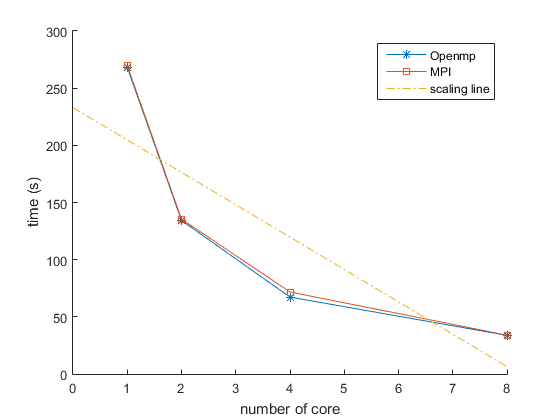
\includegraphics[width=8cm]{p11.png}
\end{figure}


The comparison between openmp and MPI,
openmp is the shared memory parallelization.
MPI is the distributed memory parallelizetion

When i do the above test, I use the machine which has 8 different cores with the shared memory.
From the computational time, we can find that the effectiveness are almost some for this two kind of parallelization due to the compute
structure.

The difference between parallel implementation is that each process has the same variables for MPI, most all of variables are shared for Openmp.

So sometime Openmp use less memory than MPI when the code is run on one single computer.

The speed of the data communication of MPI sometimes is very slower than the speed of CPU, which means we need to appropriate choose the communication function not very too much or too less
depending on the machine and the problem. Openmp is not so complexity.










\newpage

\section*{The MPI version - {red parts means what i have modified}}


Firstly,  i post the revised program,  the red sentences is the part i added.


















{\tiny{\begin{alltt}
  program main
!
 {\color{red}{ use mpi}}

  implicit none

  integer ( kind = 4 ), parameter :: nd = 3
  integer ( kind = 4 ), parameter :: np = 1000

  real ( kind = 8 ) acc(nd,np)
  real ( kind = 8 ) box(nd)
  real ( kind = 8 ), parameter :: dt = 0.0001D+00
  real ( kind = 8 ) e0
  real ( kind = 8 ) force(nd,np), {\color{red}{loc_force(nd,np)}}
  integer ( kind = 4 ) id
  real ( kind = 8 ) kinetic, {\color{red}{loc_kinetic}}
  real ( kind = 8 ), parameter :: mass = 1.0D+00
  real ( kind = 8 ) pos(nd,np)
  real ( kind = 8 ) potential , {\color{red}{loc_potential}}
  integer ( kind = 4 ) proc_num
  integer ( kind = 4 ) seed
  integer ( kind = 4 ) step
  integer ( kind = 4 ), parameter :: step_num = 400
  integer ( kind = 4 ) step_print
  integer ( kind = 4 ) step_print_index
  integer ( kind = 4 ) step_print_num
  integer ( kind = 4 ) thread_num
  real ( kind = 8 ) vel(nd,np)
  real ( kind = 8 ) wtime
 {\color{red} {real(kind=8):: loc_pos(nd,np), loc_vel(nd,np), loc_acc(nd,np)}}

 {\color{red}{ integer(kind=4)::ierr, myrank, numprocs
  integer status(MPI_STATUS_SIZE)
!
!  Initialize MPI.
!
  call MPI_Init ( ierr )
!
!  Get this process's ID.
!
  call MPI_Comm_rank ( MPI_COMM_WORLD, myrank, ierr )
!
!  Find out how many processes are available.
!
  call MPI_Comm_size ( MPI_COMM_WORLD, numprocs, ierr )

  call timestamp ( )

  wtime = MPI_Wtime ( )}}

!
!  Set the dimensions of the box.
!
  box(1:nd) = 10.0D+00
!
!  Set initial positions, velocities, and accelerations.
!
  write ( *, '(a)' ) ' '
  write ( *, '(a)' ) '  Initializing positions, velocities, and accelerations.'

  seed = 123456789
  call initialize ( np, nd, box, seed, pos, vel, acc )
!
!  Compute the forces and energies.
!
  write ( *, '(a)' ) ' '
  write ( *, '(a)' ) '  Computing initial forces and energies.'

 {\color{red}{call compute ( np, nd, pos, vel, mass, loc_force, loc_potential, loc_kinetic,myrank,numprocs )
 call MPI_Allreduce(loc_force, force,nd*np , MPI_Double, MPI_SUM,  MPI_COMM_WORLD, ierr)
 call MPI_Allreduce(loc_potential, potential, 1  , MPI_Double, MPI_SUM,  MPI_COMM_WORLD, ierr)
 call MPI_Allreduce(loc_kinetic, kinetic, 1  , MPI_Double, MPI_SUM, MPI_COMM_WORLD, ierr)}}

!

!  Save the initial total energy for use in the accuracy check.
!
  e0 = potential + kinetic
!
!  This is the main time stepping loop:
!    Compute forces and energies,
!    Update positions, velocities, accelerations.
!
  step_print = 0
  step_print_index = 0
  step_print_num = 10

  step = 0
if(myrank ==0) then
  write ( *, '(2x,i8,2x,g14.6,2x,g14.6,2x,g14.6)' ) &
    step, potential, kinetic, ( potential + kinetic - e0 ) / e0
  step_print_index = step_print_index + 1
  step_print = ( step_print_index * step_num ) / step_print_num
endif

  do step = 1, step_num

 {\color{red}{call compute ( np, nd, pos, vel, mass, loc_force, loc_potential, loc_kinetic,myrank,numprocs )
 call MPI_Allreduce(loc_force, force,nd*np , MPI_Double, MPI_SUM,  MPI_COMM_WORLD, ierr)
 call MPI_Allreduce(loc_potential, potential, 1  , MPI_Double, MPI_SUM,  MPI_COMM_WORLD, ierr)
 call MPI_Allreduce(loc_kinetic, kinetic, 1  , MPI_Double, MPI_SUM, MPI_COMM_WORLD, ierr)}}

{\color{red}{if (myrank ==0 )  then}}
  if ( step == step_print ) then

      write ( *, '(2x,i8,2x,g14.6,2x,g14.6,2x,g14.6)' ) &
        step, potential, kinetic, ( potential + kinetic - e0 ) / e0

      step_print_index = step_print_index + 1
      step_print = ( step_print_index * step_num ) / step_print_num

    end if
{\color{red}{endif}}

 {\color{red}{   call update ( np, nd,loc_pos, loc_vel, loc_acc,  pos, vel, force, acc, mass, dt, myrank, numprocs )
    call MPI_Allreduce(loc_pos,pos, nd*np , MPI_Double, MPI_SUM,  MPI_COMM_WORLD, ierr)
    call MPI_Allreduce(loc_vel,vel, nd*np , MPI_Double, MPI_SUM,  MPI_COMM_WORLD, ierr)
    call MPI_Allreduce(loc_acc,acc, nd*np , MPI_Double, MPI_SUM,  MPI_COMM_WORLD, ierr)}}


  end do
{\color{red}{if(myrank ==0 ) then
  wtime = MPI_Wtime ( ) - wtime}}
  write ( *, '(a)' ) ' '
  write ( *, '(a)' ) '  Elapsed time for main computation:'
  write ( *, '(2x,g14.6,a)' ) wtime, ' seconds'
!
!  Terminate.
!
  write ( *, '(a)' ) ' '
  write ( *, '(a)' ) 'MD_OPENMP'
  write ( *, '(a)' ) '  Normal end of execution.'

  write ( *, '(a)' ) ' '
  call timestamp ( )

 {\color{red}{endif
  call MPI_Finalize ( ierr )}}
  stop
end
subroutine compute ( np, nd, pos, vel, mass, f, pot, kin ,{\color{red}{myrank, numprocs }})
!
  implicit none

  integer ( kind = 4 ) np, {\color{red}{numprocs, myrank}}
  integer ( kind = 4 ) nd

  real ( kind = 8 ) d
  real ( kind = 8 ) d2
  real ( kind = 8 ) f(nd,np)
  integer ( kind = 4 ) i
  integer ( kind = 4 ) j
  real ( kind = 8 ) kin
  real ( kind = 8 ) mass
  real ( kind = 8 ), parameter :: PI2 = 3.141592653589793D+00 / 2.0D+00
  real ( kind = 8 ) pos(nd,np)
  real ( kind = 8 ) pot
  real ( kind = 8 ) rij(nd)
  real ( kind = 8 ) vel(nd,np)

  pot = 0.0D+00
  kin = 0.0D+00


 {\color{red}{ do i = myrank+1, np, numprocs}}
!
!  Compute the potential energy and forces.
!
    f(1:nd,i) = 0.0D+00

    do j = 1, np

      if ( i /= j ) then

        call dist ( nd, pos(1,i), pos(1,j), rij, d )
!
!  Attribute half of the potential energy to particle J.
!
        d2 = min ( d, PI2 )

        pot = pot + 0.5D+00 * ( sin ( d2 ) )**2

        f(1:nd,i) = f(1:nd,i) - rij(1:nd) * sin ( 2.0D+00 * d2 ) / d

      end if

    end do
!
!  Compute the kinetic energy.
!
    kin = kin + sum ( vel(1:nd,i)**2 )

  end do


  kin = kin * 0.5D+00 * mass

  return
end

subroutine update ( np, nd, {\color{red}{loc_pos, loc_vel, loc_acc,}} pos, vel, f, acc, mass, dt, {\color{red}{myrank, numprocs }})
!call update ( np, nd, pos, vel, force, acc, mass, dt, myrank, numprocs )
!
  implicit none

  integer ( kind = 4 ) np
  integer ( kind = 4 ) nd

  real ( kind = 8 ) acc(nd,np)
  real ( kind = 8 ) dt
  real ( kind = 8 ) f(nd,np)
  integer ( kind = 4 ) i
  integer ( kind = 4 ) j
  real ( kind = 8 ) mass
  real ( kind = 8 ) pos(nd,np)
  real ( kind = 8 ) rmass
  real ( kind = 8 ) vel(nd,np)
  {\color{red}{integer(kind=8) myrank, numprocs}}
  {\color{red}{real(kind=8):: loc_pos(nd,np), loc_vel(nd,np), loc_acc(nd,np)}}
  rmass = 1.0D+00 / mass
 {\color{red}{ loc_pos = 0.0d0
  loc_vel = 0.0d0
  loc_acc = 0.0d0}}
  {\color{red}{do j = myrank + 1, np, numprocs}}
    do i = 1, nd
      {\color{red}{loc_pos(i,j)}} = pos(i,j) + vel(i,j) * dt + 0.5D+00 * acc(i,j) * dt * dt
      {\color{red}{loc_vel(i,j)}} = vel(i,j) + 0.5D+00 * dt * ( f(i,j) * rmass + acc(i,j) )
      {\color{red}{loc_acc(i,j)}} = f(i,j) * rmass
    end do
  {\color{red}{end do}}

  return
end

\end{alltt}}}






\end{document}
